% file: reasoning_case.tex

\begin{ReasoningBox}[title=Domain Knowledge Error] % 可以通过 title 参数修改标题
    % --- 第一部分：问题描述与图片 ---
    % \begin{minipage}[t]{0.58\textwidth}
    \begin{wrapfigure}{r}{0.5\textwidth}
        \centering
        % wrapfigure 通常顶部会有多余空白，使用负 vspace 向上提，让图片和第一行文字对齐
        \vspace{-15pt} 
        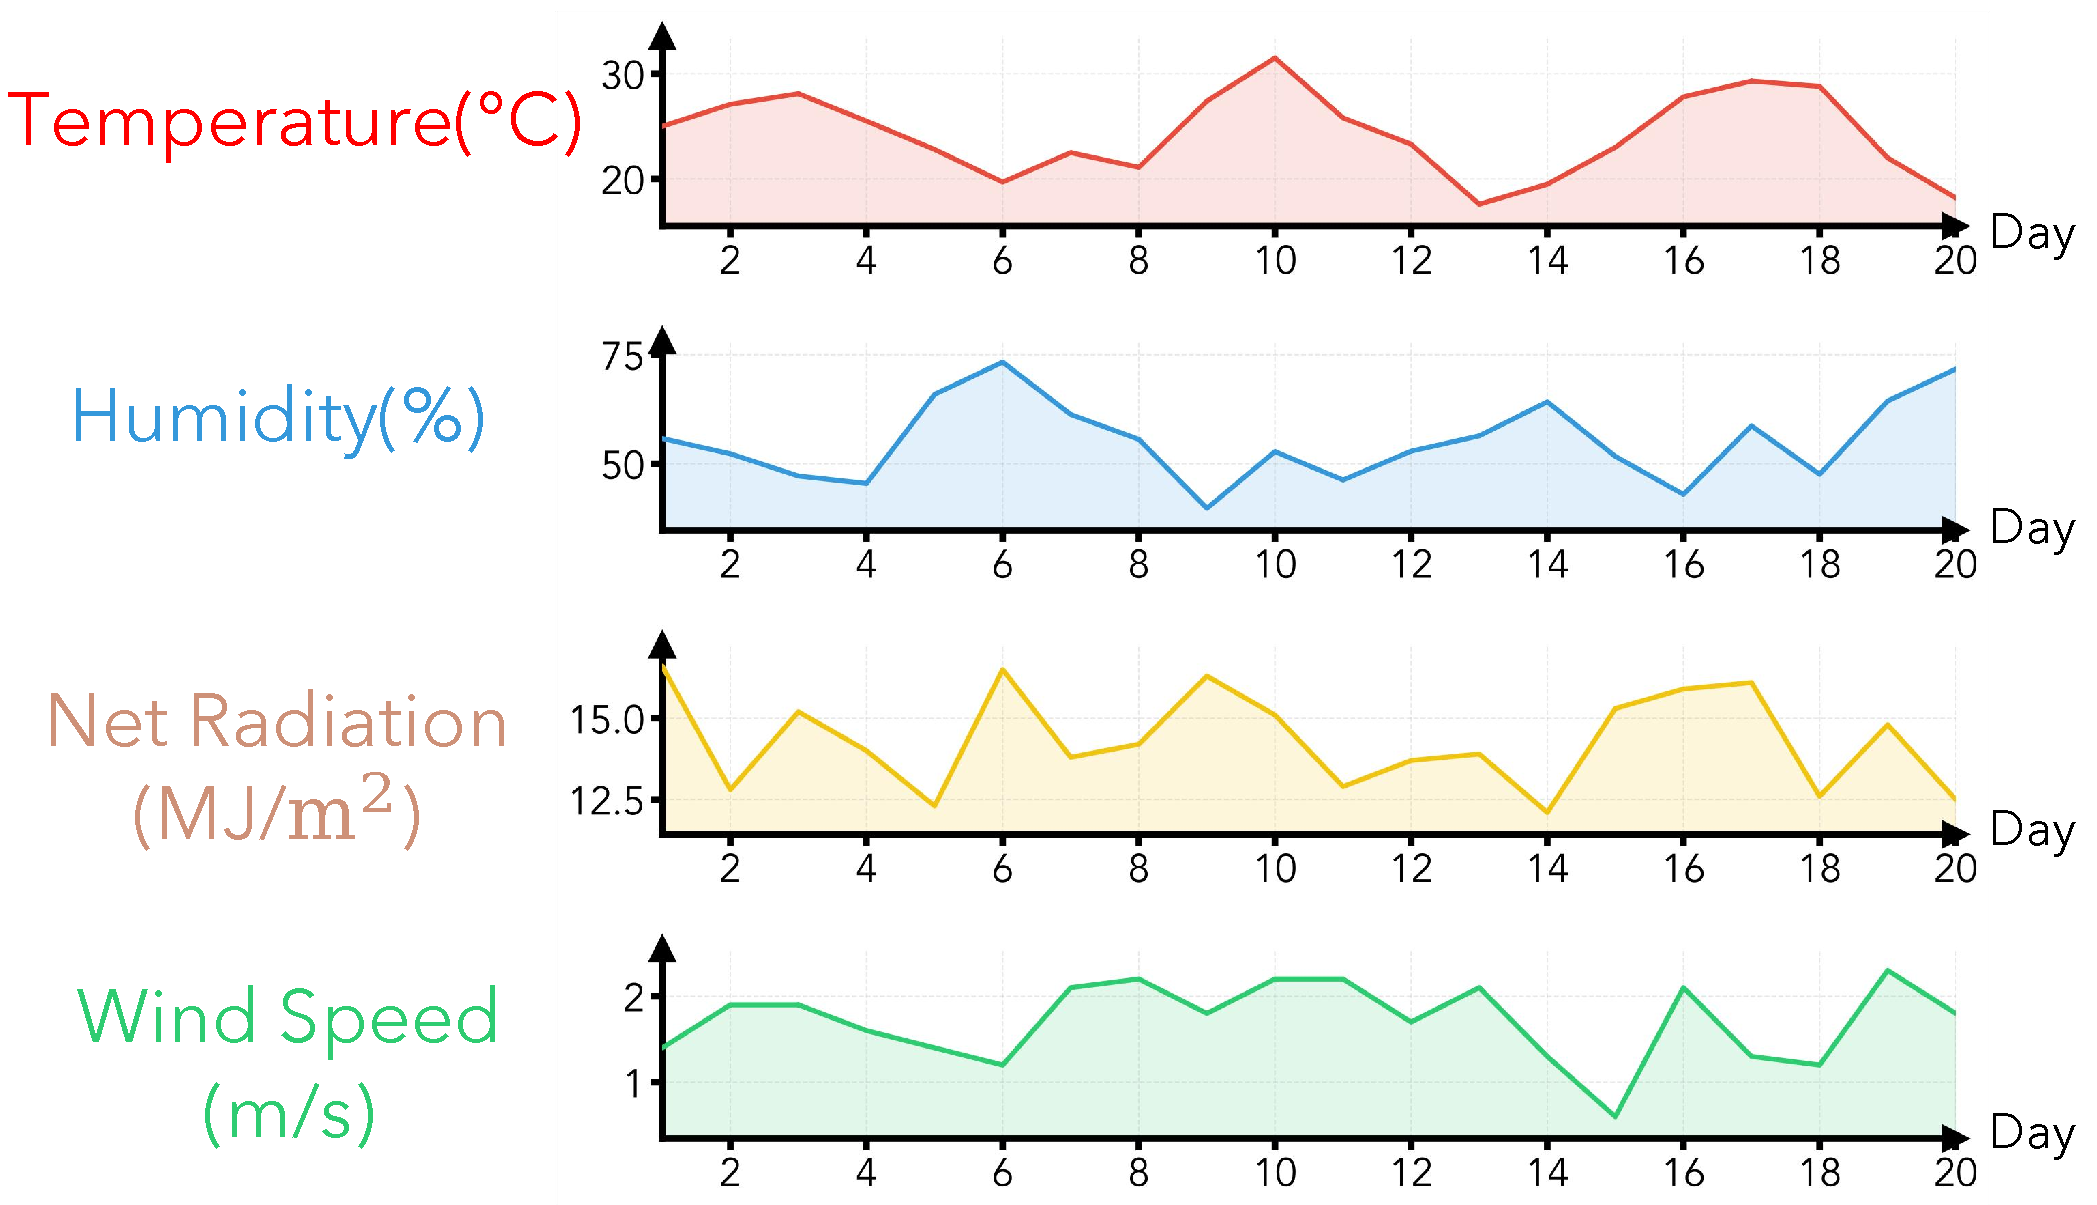
\includegraphics[width=\linewidth]{blocks/case_study_figs/knowledge_error.pdf}
        % 调整底部的留白
        \vspace{-10pt}
    \end{wrapfigure}
        \textbf{Question:} The following time series shows daily meteorological data: temperature ($^\circ$C), relative humidity (\%), net radiation (MJ/m$^2$/day), and wind speed at 2m height (m/s). Using the \textbf{FAO-56 Penman-Monteith equation}, what is the \textbf{total cumulative reference evapotranspiration ($ET_0$)} over this period (in mm)?
    % \end{minipage}%
    % \hfill
    

    \vspace{0.5em}

    % --- 第二部分：选项 ---
    \textbf{Answer Choices:} (A) 67.9, (B) 116.5, (C) 166.4, (D) 216.3 \\
    \textbf{Correct Answer:} \textcolor{correctgreen}{(C)} \\
    \textbf{Model Answer:} \textcolor{wrongred}{(D)}
    
    \vspace{0.3em}

    % --- 第四部分：基本原理 (Rationale) ---
    \textbf{Prediction Rationale:} To calculate the total cumulative reference evapotranspiration ($ET_0$) using the FAO-56 Penman-Monteith equation, we apply the formula for each day and sum the results. The equation used is:
    \[
    ET_0 = \frac{0.408\Delta(R_n - G) + \gamma \times (900 / (T + 273)) \times u_2 \times \text{VPD}}{\Delta + \gamma}
    \]
    where $ET_0$ is in mm/day, $\Delta$ is slope of vapor pressure curve, $R_n$ is net radiation, $G\approx0$, $\gamma=0.067$, $T$ is temp, $u_2$ is wind speed, and VPD is vapor pressure deficit.
    
    \textbf{Estimation from graph:}
    We estimated daily values for 25 days. For example:
    \begin{itemize}
        \item Day 0: $T\approx28^\circ$C, $RH\approx50\%$, $R_n\approx13.5$, $u_2\approx3.0$. Calculated $ET_0 \approx 8.22$ mm/day.
        \item Average conditions: $T\approx25^\circ$C, $RH\approx50\%$, $R_n\approx13.5$, $u_2\approx3.0$.
    \end{itemize}
    
    \textbf{Calculation:}
    Using average values ($T=25^\circ$C), we computed $ET_0 \approx 7.66$ mm/day. Total over 25 days $\approx 191.5$ mm.
    Sensitivity check with higher temperatures:
    \begin{itemize}
        \item At $T=29^\circ$C: $ET_0 \approx 8.31$ mm/day $\rightarrow$ Total $\approx 207.75$ mm.
        \item At $T=30^\circ$C: $ET_0 \approx 8.40$ mm/day $\rightarrow$ Total $\approx 210.0$ mm.
    \end{itemize}
    Given temperatures often exceed $28^\circ$C and high radiation, the total is likely around 215--220 mm. Option D (216.3) matches this estimate best. \\
    \par            % 确保结束上一段
    % \vspace{0.8em}  % 调整上方留白
    \hrule          % 绘制横线
    \vspace{0.8em}  % 调整下方留白
    \textbf{Error Analysis:} \textit{The model systematically overestimated the result due to a **domain knowledge error** in the formula application. It used an incorrect denominator ($\Delta + \gamma$) instead of the standard FAO-56 form ($\Delta + \gamma(1 + 0.34u_2)$). By omitting the wind speed correction term ($1 + 0.34u_2$), the model significantly underestimated the aerodynamic resistance, inflating daily $ET_0$ values by approx. 27\%, pushing the cumulative total from 166.4 mm (Ground Truth) to 216.3 mm (Model's choice).}
\end{ReasoningBox}